%% This work is distributed under the LaTeX Project Public License (LPPL)
%% ( http://www.latex-project.org/ ) version 1.3, and may be freely used,
%% distributed and modified. A copy of the LPPL, version 1.3, is included
%% in the base LaTeX documentation of all distributions of LaTeX released
%% 2003/12/01 or later.
%% Retain all contribution notices and credits.
%% ** Modified files should be clearly indicated as such, including  **
%% ** renaming them and changing author support contact information. **
%%*************************************************************************
\documentclass[conference]{IEEEtran}
\usepackage{xcolor}
\usepackage{hyperref}
\usepackage{graphicx}
\usepackage{float}
\definecolor{linkcolor}{HTML}{0000FF} % цвет ссылок
\definecolor{urlcolor}{HTML}{0000FF} % цвет гиперссылок
\hypersetup{pdfstartview=FitH, citecolor = Black, linkcolor=linkcolor,urlcolor=urlcolor, colorlinks=true}

\usepackage{fontspec}
\setmainfont[
 Path = ./ ,
 Extension = .otf ,
 Mapping=tex-text,
 Ligatures={TeX, Common},
 BoldFont = texgyretermes-bold,
 ItalicFont = texgyretermes-italic,
 BoldItalicFont = texgyretermes-bolditalic,
 SmallCapsFont = texgyretermes,
 SmallCapsFeatures = {Letters = SmallCaps}
]{texgyretermes}

\usepackage{polyglossia}
\setdefaultlanguage{russian}
\setotherlanguages{english}

\usepackage[backend=biber,style=ieee,refsection=section]{biblatex}    
% *** CITATION PACKAGES ***
%
% \usepackage{cite}
% cite.sty was written by Donald Arseneau
% V1.6 and later of IEEEtran pre-defines the format of the cite.sty package
% \cite{} output to follow that of the IEEE. Loading the cite package will
% result in citation numbers being automatically sorted and properly
% "compressed/ranged". e.g., [1], [9], [2], [7], [5], [6] without using
% cite.sty will become [1], [2], [5]--[7], [9] using cite.sty. cite.sty's
% \cite will automatically add leading space, if needed. Use cite.sty's
% noadjust option (cite.sty V3.8 and later) if you want to turn this off
% such as if a citation ever needs to be enclosed in parenthesis.
% cite.sty is already installed on most LaTeX systems. Be sure and use
% version 5.0 (2009-03-20) and later if using hyperref.sty.
% The latest version can be obtained at:
% http://www.ctan.org/pkg/cite
% The documentation is contained in the cite.sty file itself.

\usepackage{graphicx}
\usepackage{amsmath}
\usepackage{url}
\usepackage{array}
\usepackage[caption=false,font=footnotesize]{subfig}
\usepackage{lipsum}
% \usepackage[caption=false,font=footnotesize]{subfig}
% \usepackage{dblfloatfix}
% The latest version can be found at:
% http://www.ctan.org/pkg/dblfloatfix

\renewcommand{\thesubsection}{\Alph{subsection}.}
\renewcommand{\thesubsubsection}{\arabic{subsubsection})}
\renewcommand{\theparagraph}{\alph{paragraph})}


% The following code makes "fake small caps" which work fine
% for cyrillic symbols
% Borrowed from http://tex.stackexchange.com/questions/64582/faking-small-caps-in-xelatex?rq=1


\usepackage{expl3,xparse}

% turn expl3 space on: `:' and `_' are letters now and spaces
% are ignored. To insert a space use `~'.
\ExplSyntaxOn
% the internal command:
\cs_new:Npn \fakecaps:n #1
  {
    \addfontfeature{LetterSpace=10.0} {\tl_head:n { #1 }\kern 1pt}{\addfontfeature{Scale=0.9}\uppercase{\tl_tail:n { #1 }}}
  }

% the document command:
\NewDocumentCommand\FakeCaps{m}
  {\fakecaps:n { #1 } }

% turn expl3 space off again:
\ExplSyntaxOff

\makeatletter
\newcommand\subparagraph{%
  \@startsection{subparagraph}{5}
  {\parindent}
  {3.25ex \@plus 1ex \@minus .2ex}
  {-1em}
  {\normalfont\normalsize\bfseries}}
\makeatother
\usepackage[explicit]{titlesec}
\let\subparagraph\relax
\titleformat{\section}[hang]{\normalfont\normalsize\centering}{\thesection.}{0.5em}{\FakeCaps{#1}}

\makeatletter
\def\russian@capsformat{}
\makeatother



% If you need to correct hyphenations, add them here
\hyphenation{op-tical net-works semi-conduc-tor}

\begin{document}
% paper title
%
% In English titles are generally capitalized except for words such as a, an, and, as,
% at, but, by, for, in, nor, of, on, or, the, to and up, which are usually
% not capitalized unless they are the first or last word of the title.
% Linebreaks \\ can be used within to get better formatting as desired.
% Do not put math or special symbols in the title.
\title{Телеметрия роботов на базе контроллера TRIK}

\author{\IEEEauthorblockN{Свитков С. А.}
\IEEEauthorblockA{Санкт-Петербургский\\Государственный Университет\\
Email: svitkovsergey@gmail.com}
\and
\IEEEauthorblockN{Железняков И. Э.}
\IEEEauthorblockA{Санкт-Петербургский\\Государственный Университет\\
Email: iz14@yandex.ru}
}

% make the title area
\maketitle

% As a general rule, do not put math, special symbols or citations
% in the abstract
\begin{abstract}
Представлен опыт сбора данных с контроллеров TRIK, возможные подходы к реализации телеметрии. В результате применения описанного в статье подхода к сбору данных с устройства среднее время передачи пакета данных уменьшилось примерно на 15\%. Приведенные в статье методы решения задачи телеметрии могут быть адаптированы для применения и на других устройствах, оснащенных Wi-Fi.
\end{abstract}

\section{Введение}
% no \IEEEPARstart
В последние годы область робототехники развивается очень быстро, появляется множество робототехнических конструкторов.


Одним из них является TRIK \cite{trik} --- кибернетический конструктор с центральным процессором на базе ARM и операционной системой на базе ядра Linux. Модели роботов TRIK применяются как для обучения школьников, так и для серьезных соревнований, например, WRO (World Robot Olympiad), проходившей в Сочи (2014г); Ежегодный фестиваль робототехники Робофинист (2015г). Роботы моделей TRIK имеют ряд датчиков, таких как гироскоп, акселерометр, датчик заряда батареи. Так же робот предоставляет сетевой интерфейс Wi-Fi.


Но сам по себе робот, без программ на нем, представляет малый интерес. Следует сказать, что исполнение программ на роботе происходит в реальном времени, поэтому очень важной является возможность отслеживать показания датчиков робота во время работы приложений. Выводить полученные данные хотелось бы в удобной для пользователя форме.
Кроме того, необходимо учитывать, что соединение Wi-Fi с роботом нестабильно, и его легко перегрузить, поэтому алгоритм обмена сообщениями между роботом и ПК должен работать быстро, но при этом обеспечивать минимальную потерю данных.


Таким образом, перед нами встала задача написания приложения, удовлетворяющего поставленным выше требованиям --- с визуализацией получаемых с робота данных и алгоритмом передачи данных, предоставляющим высокую скорость обмена информацией между клиентом и сервером при минимальных потерях показаний датчиков. Так как работа выполняется в условиях реального времени, алгоритм должен обеспечивать поступление данных на клиентскую часть с минимальной задержкой. Данный алгоритм и является основной темой статьи. Для его реализации была использована комбинация протоколов передачи данных TCP и UDP, так как TCP предоставляет надежное соединение, предотвращающее потерю пакетов с данными, для передачи важных сигналов, а UDP --- высокую скорость для передачи большого количества данных с датчиков робота. Описанный в статье подход может быть обобщен и использован для решения других задач, в частности, для других контроллеров или для IoT \cite{IOT}.


Проблема высокоскоростной передачи данных и минимальными потерями пакетов при слабом сигнале сети не является новой, существует несколько решений, описанных в различных научных статьях, публиковавшихся ранее.

\section{Обзор существующих решений}

\subsection{A Comparison of Lightweight Communication Protocols in Robotic Applications}

В данной статье \cite{paper1} производится сравнение двух легковесных протоколов передачи данных : CoAP \cite{coap} и MQTT-SN \cite{mqtt}.
Оба протокола могут использовать UDP в качестве своей основы. 

Приведенный в нашей статье алгоритм использует чистые TCP и UDP протоколы, без каких-либо надстроек над ними. В ходе дальнейшей работы над приложением планируется протестировать иные варианты передачи данных и сравнить их с нашим решением.

\subsection{A Data-Rate Aware Telemetry Scheduler}

Данная статья \cite{paper2} рассказывает о проблеме передачи данных с робота в условиях очень плохого соединения. Приведенный в статье алгоритм основывается на актуальности сообщений --- сообщения с данными передаются не в том порядке, в котором данные были получены роботом, а в том, который соответствует актуальности каждого сообщения.

Задача, поставленная в нашей статье, отличается тем, что критически важные данные всегда передаются по TCP, а менее важные - по UDP. 

\section{Клиентская часть}
Для реализация клиента был выбран язык C++ и библиотека Qt \cite{qt}, так как система сигналов и слотов в Qt очень удобна для решения данной задачи. 


\subsection{Архитектура}
Архитектура клиента \ref{overflow1} спроектирована с помощью паттернов проектирования \cite{gof}.

\begin{figure*}
\centering
\includegraphics[width=\textwidth]{/home/likeanowl/Downloads/client}
\caption{Архитектура клиентской части \label{overflow1}}
\end{figure*}

Панель управления реализована с применением паттерна Model View Controller.


Для упрощения доступа к логической части программы использован паттерн Facade, то есть все запросы и вызовы внешнего кода сведены к одному объекту, причем внешний код не знает, как именно эти запросы обрабатываются.


В системе отображения показаний датчиков используется паттерн Observer. Пользователю предоставлена возможность вывода на экран нескольких виджетов для визуализации одних и тех же данных (с помощью графика, в табличном виде и так далее). При создании класса, отвечающего за отрисовку конкретного виджета, класс виджета обращается к объекту, хранящему соответствующие показания, и подписывается на получение их обновлений.
Клиент получает данные с сервера по одному из протоколов (TCP, UDP), каждый из протоколов реализован в отдельном классе, наследуемом от общего интерфейса. 


Полученная информация в виде названий датчиков и их показаний передается в класс Parser, где происходит разбор данных, затем по идентификатору сенсора отправляется в соответствующий класс для хранения. 
\subsection{Применение виджетов}
Все виджеты реализованы как перемещаемые по рабочей области элементы QDockWidget, содержащие в себе виджеты визуализации. Для отрисовки графиков как наиболее оптимальная была выбрана библиотека QCustomPlot \cite{qcustomplot} с открытым исходным кодом.


При желании пользователя отобразить показания датчика с помощью системы сигналов и слотов Qt производится определенный запрос данных у объекта, хранящего показания, после чего они отображаются в выбранном пользователем виде на отдельном виджете. Вместе с закрытием виджета происходит его отписка от получения новых данных со стороны класса, содержащего показания сенсоров.


Отрисовка каждого виджета на форме происходит с заранее заданным периодом, а не по изменению показаний. Сделано это для того, чтобы уменьшить нагрузку при рисовании и сделать отрисовку независимой от скорости передачи данных по сети Wi-Fi.

\section{Серверная часть}

Для реализации серверной части приложения был выбран язык C++ с фреймворком Qt. Основной интерес в реализации сервера представляют два момента : снятие показаний с датчиков робота и алгоритм их передачи.

\begin{figure*}
\centering
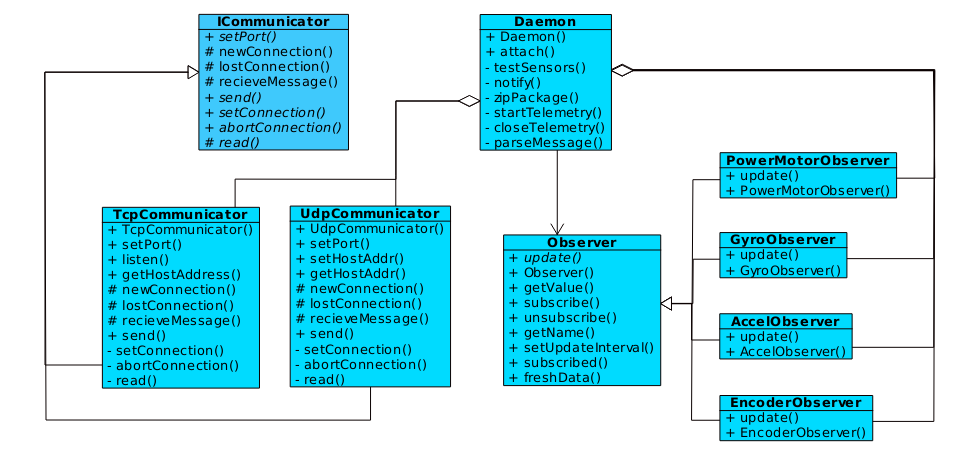
\includegraphics[width=\textwidth]{/home/likeanowl/Downloads/serv}
\caption{Архитектура серверной части \label{overflow2}}
\end{figure*}

\subsection{Снятие показаний}
Данные с датчиков робота снимаются с помощью библиотеки trikControl - части TrikRuntime. TrikRuntime \cite{trikruntime} --- среда выполнения для TRIK с открытым кодом, предоставляющая следующие средства для работы с контроллером : 
\begin{itemize}
\item trikControl --- библиотека для работы с аппаратной частью робота, предоставляющая интерфейс для аппаратной части в виде Qt классов
\item trikScriptRunner --- библиотека, предоставляющая интерпретатор QtScript, в результате позволяя использовать trikControl при исполнении файлов QtScript
\item trikCommunicator --- библиотека, предоставляющая сетевой интерфейс для запуска программ на роботе
\item trikRun --- консольная утилита для запуска файлов \cite{qtscript} QtScript
\item trikServer --- консольная утилита для поднятия сервера для обмена данными по сети
\item trikGui --- графический интерфейс
\item trikKernel --- библиотека с общим кодом для всех остальных проектов
\end{itemize} 
Для отслеживания показаний всех датчиков используется архитектурное решение \ref{overflow2}, в котором применен паттерн Observer - объекты, хранящие показания датчиков, подписываются на получение обновлений показаний датчиков и следят за ними, а при сигнале с клиентской части о завершении телеметрии - отписываются от обновлений и перестают сохранять информацию. Снятие показаний с датчиков происходит каждые 10 мс.


Объекты-наблюдатели хранятся в списке, и при получении сигнала с клиентской части о начале телеметрии данные, хранящиеся в каждом наблюдателе, переводятся в строку, которая отправляется на клиент с помощью алгоритма, описанного ниже.
\subsection{Реализация передачи данных}
Реализация передачи данных является наиболее интересной частью работы над сервером. Обмен данными осуществляется по двум протоколам --- TCP и UDP. Использование комбинации протоколов TCP и UDP для обмена данными дает большую скорость их передачи, чем использование только протокола TCP, и большую надежность, чем использование только протокола UDP.
\begin{itemize}
\item TCP --- протокол, обеспечивающий сохранность данных при передаче за счет предварительной установки соединения и осуществления повторого запроса в случае потери части пакетов. Таким образом гарантируется целостность передаваемых данных и уведомление отправителя о том, что данные были получены.


Поэтому TCP в данном случае используется для обмена сервера и клиента сигналами такими, как сигнал о старте телеметрии, сигнал о ее завершении. Поскольку подобные сообщения передаются сравнительно нечасто, медленная скорость работы TCP не оказывает большого влияния на общую скорость передачи данных.
\item UDP --- протокол, в отличие от TCP, не обеспечивающий сохранность данных при передаче. Поскольку передача данных осуществляется в режиме реального времени, объем данных большой, а частота отправки высокая, потеря некоторой части не будет существенна. Но скорость передачи и нагрузка на сеть будут ниже, чем при использовании TCP 
\end{itemize}
Таким образом, использование и TCP, и UDP является оптимальным для данной задачи.

При работе сервера сначала определяется тип данных, которые должны быть переданы на клиент, сообщение конвертируется в массив байт. После этого, в зависимости от типа передаваемого сообщения, выбирается способ его передачи --- TCP или UDP.


Были произведены замеры скорости передачи данных, результаты которых указаны в таблице \ref{tab:table1}

\begin{table}
\centering
  \caption{Результаты замеров}
  \label{tab:table1}
  \begin{tabular}{|p{1.3 cm}|p{1 cm}|p{1.7 cm}|p{1 cm}|p{1.5 cm}|}
    \hline
    Количество отправляемых пакетов & Размер одного пакета, байт & Используемый протокол & Среднее время передачи, мс & Среднекв. отклонение для выборки из 100 замеров, мс\\
    \hline
    1000 & 75 & TCP & 13213.2 & 177.5\\
    \hline
    1000 & 75 & TCP + UDP & 11987.8 & 82.1\\
    \hline
    10000 & 75 & TCP & 133414.6 & 274.1 \\
    \hline 
    10000 & 75 & TCP + UDP & 119058.6 & 121.9 \\
    \hline
    500 & 375 & TCP & 16910.6 & 148.3 \\
    \hline
    500 & 375 & TCP + UDP & 15129.2 & 111.8 \\
    \hline
    500 & 150 & TCP & 9249.3 & 132.2 \\
    \hline
    500 & 150 & TCP + UDP & 7976.4 & 46.1 \\
    \hline
  \end{tabular}
\end{table}
\\

Были произведены замеры количества пакетов, теряемых при использовании TCP + UDP, данные указаны в таблице \ref{tab:table2}. По результатам, представленным в таблице, можно заметить, что количество потерянных при передаче по UDP пакетов составляет около 20\% от общего числа. Несмотря на то, что такой процент потерянных пакетов может казаться большим,
это не существенно, так как 1 пакет с данными передается каждые 10 мс, а клиентская часть при отсутствии новых пакетов продолжает визуализировать последние полученные данные.

\begin{table}
\centering
  \caption{Результаты замеров}
  \label{tab:table2}
  \begin{tabular}{|p{1.5 cm}|p{1.5 cm}|p{1.5 cm}|}
    \hline
	Количество отправляемых пакетов & Среднее количество терямых пакетов & Среднекв. отклонение для выборки из 100 \\
	\hline
	10000 & 2076.4 & 153.23 \\
	\hline
	1000 & 196.7 & 30.1 \\
	\hline
  \end{tabular}
\end{table}
\\
\section{Заключение}
Результатом работы является клиент-серверное приложение для сбора и визуализации данных с использованием двух протоколов для обмена данными между клиентом и сервером. Приведенное решение задачи телеметрии позволяет увеличить скорость обмена данными в среднем на 15\%, что позволяет передавать большее количество данных, не теряя их актуальности. Использование TCP для передачи важных сообщений гарантирует их сохранность. Приведенное решение визуализирует данные, получаемые с робота, в удобной для пользователя форме. 

В планах дальнейшей работы --- добавление визуализации новых типов данных в клиентскую часть, разбиение работы сервера на несколько потоков для достижения большей скорости работы, улучшение алгоритма сжатия передаваемых сообщений с целью уменьшения нагрузки на сеть.

Идея использования двух протоколов для обмена данными может быть обобщена и успешно применена в других проектах, требующих одновременно и быстродействия, и минимальных потерь информации.

%\clearpage
\begin{thebibliography}{1}

  \bibitem{trik} Домашняя страница проекта TRIK, URL : \url{http://www.trikset.com/} Дата обращения : 29.02.2016 \\

  \bibitem{IOT} Internet of Things, URL : \url{https://en.wikipedia.org/wiki/Internet_of_Things} Дата обращения : 14.04.2016 \\

  \bibitem{paper1} A Comparison of Lightweight Communication Protocols in Robotic Applications, URL : \url{http://www.sciencedirect.com/science/article/pii/S1877050915038193} Дата обращения : 14.04.2016 \\
  
  \bibitem{coap} CoAP, URL : \url{https://en.wikipedia.org/wiki/Constrained_Application_Protocol} Дата обращения : 14.04.2016 \\
  
  \bibitem{mqtt} MQTT, URL : \url{https://en.wikipedia.org/wiki/MQTT} Дата обращения : 14.04.2016 \\
  
  \bibitem{paper2} A Data-Rate Aware Telemetry Scheduler, URL : \url{https://www.ri.cmu.edu/publication_view.html?pub_id=3734} Дата обращения : 14.04.2016 \\

  \bibitem{qt} Библиотека Qt, URL : \url{http://qt.io} Дата обращения : 29.02.2016 \\

  \bibitem{gof} Erich Gamma, Richard Helm, Ralph Johnson, John Vlissides, Design Patterns: Elements of Reusable 			Object-Oriented Software, 416 pp., Addison Wesley, 1994 

  \bibitem{qcustomplot} Библиотека QCustomPlot, URL : \url{http://www.qcustomplot.com/} Дата обращения : 29.02.2016 \\

  \bibitem{trikruntime} Документация среды выполнения TrikRuntime, URL : \url{https://github.com/trikset/trikRuntime/wiki} Дата обращения : 29.02.2016 \\ 

  \bibitem{qtscript} Документация QtScript, URL : \url{http://doc.qt.io/qt-5/qtscript-index.html} Дата обращения : 29.02.2016 \\

\end{thebibliography}

\end{document}


